\subsection{RSA Accumulator}

Recall idea of RSA accumulator. Given hash function $H : \{0, 1\}^* \rightarrow
\mathbb{N}$, generating only primes.

\begin{algorithm}
		\caption{RSA accumulatlr}

        \begin{algorithmic}[0]
				\Procedure{KeyGen}{}
                  \State $p, q$ primes
                  \State $N \coloneqq p \cdot q$
                  \State $sk \coloneqq \varphi(N) = (p - 1) (q - 1)$
                  \State $pk \coloneqq N$
                  \State \textbf{Return} $(pk, sk)$
                \EndProcedure

                \Procedure{Init}{$N, X$}
                  \State $(x_1, \ldots, x_n) \rightarrow x$ \Comment{Secret-sharing}
                  \State $r \rgets \mathbb{Z}_N$
                  \State $\alpha \coloneqq r^{\prod H(i || x_i)} \mod N$
                  \For{$i = 1$ to $n$}
                    \State $w_i \coloneqq \alpha^{\frac{i}{H(i || x_i)}} \mod N$ \Comment{Secret key needed to calculate inverse of hash}
                  \EndFor
                  \State \textbf{Return} $((x_1, \ldots, x_n; w_1, \ldots, w_n), \alpha)$ \Comment{$w_i$ is wittness for $x_i$}
                \EndProcedure

                \Procedure{Query}{$\overline{x}, \alpha, q$} \Comment{Where $q$ is $\operatorname{read}(i)$}
                  \State \textbf{Return} $(x_i, w_i)$
                \EndProcedure

                \Procedure{Verify}{$N, \alpha, q, x_i, w_i$}
                  \State \textbf{Return} $w_i^{H(i || x_i)} \equiv \alpha \pmod{N}$
                \EndProcedure

                \Procedure{Update}{$sk, \overline{x}, \alpha, u$} \Comment{Where $u$ is $\operatorname{write}(i, v)$}
                  \State $\alpha' \coloneqq \alpha^{\frac{1}{H(i || x_i)} \cdot H(i || v)} \mod N$ \Comment{Inversion of hash needs sk}
                  \State Update or recompute all wittnesses $w_1, \ldots, w_n$
                  \State \textbf{Return} $(i, v, (w_1, \ldots, w_n), \alpha')$
                \EndProcedure

                \Procedure{Refresh}{$pk, \overline{x}, \alpha', u$}
                  \State $x_i \coloneqq v$
                  \State Recompute all wittnesses
                  \For{$i = 1$ to $n$}
                    \State $w_i \coloneqq r^{\prod_{j=1, j \neq i}^n H(j || x_j)} \pmod{N}$ \Comment{This is expensive}
                  \EndFor
                \EndProcedure
        \end{algorithmic}
\end{algorithm}

Note that $\alpha$ authenticates the whole (unordered) set $(x_i)$, and $w_i$ a
specific $x_i$.

\subsubsection{Properties}

\begin{description}
  \item[Completness] Directly from $w_i^{H(i || x_i)} \equiv \alpha^1 \equiv
    \alpha \pmod{N}$
  \item[Security] If adversary managed to produce $\hat{x_i}, \hat{w_i}$ with
    $\hat{x_i} \neq x_i$ such that it passes verification, then $\hat{w_i}^{H(i
    || \hat{x_i})}$ which would contradict the strong RSA assumption.
  \item[Efficiency (operations)] Query and verify take constant number of
    operations. Update and refresh take $O(n)$.
  \item[Efficiency (storage)] $O(n)$ extra space
\end{description}

\subsection{Trivial authenticated data structure}

\begin{itemize}
  \item Writer signs every value $x_i$
  \item Signatures stored at server $S$
  \item Timestamp $ts$ ensures freshness, prevents replay attacks. Timestamp
    counts number of write operations.
  \item Each update signs again all $x_i$ as $\sigma_i \coloneqq \operatorname{sign}(sk, i || ts || x_i)$
\end{itemize}

\subsection{Comparison of ADS}

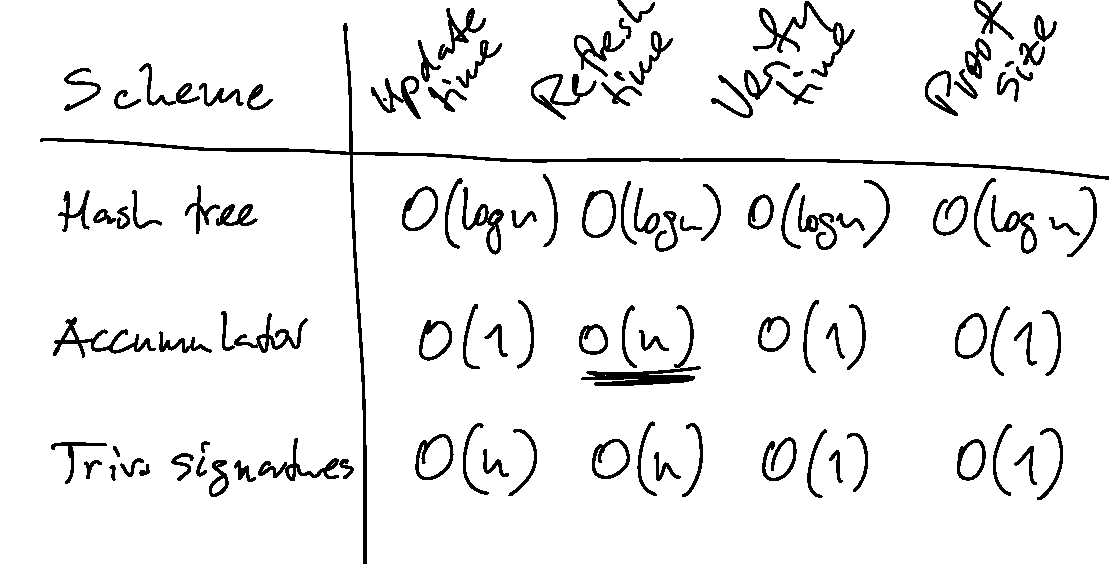
\includegraphics[width=\textwidth]{14_comparison}
